\chapter{Testing the  Stability of the Stock Market}
\label{Chap:Framework}

\section{Introduction}

This chapter answerers the question of capability of being able to generalise the use of the temporal rule-based classification which is proposed to classify players of the public goods game. In this chapter, we will check the validity of Hypothesis  \ref{hypo:pridictabilityOfStocks} regarding stock market predictability by classifying them into different stability classes. To be able to classify a larger data than public goods game, a heuristic algorithm has to be used for optimising the initial rules instead of enumerating all possible rule combinations.

In this chapter we will validate Hypothesis \ref{hypo:pridictabilityOfStocks} by classifying stock market data set for two consecutive quarters of the financial year and then comparing an individual stock's stability classes. The hypothesis indicates that to be able to predict the stock market, at least half of the stocks should follow the same stability class. We also use the proposed method in chapter four for measuring changes over time to determine the stability of the stock markets using different reference of behaviours.

The presented stock market data set of  S\&P\,500 in chapter three is classified to validate Hypothesis \ref{hypo:pridictabilityOfStocks}. The stocks are classified into four different stability classes: very stable; smooth stable; rough stable; and unstable. Profiles for each stock are created to construct the initial rules and determine the [min, max] range of the rule values. 

For optimisation process, we use the differential evolution algorithm, which is developed by Storn et al.  \cite{Storn1997}, as a heuristic function to improve the speed of the process. To check the efficiency of the differential evolutionary algorithm, we compare the brute force results of the public goods games data sets with the heuristic results. Then, the classification results of the proposed method for the public goods games will be compared with common classification algorithms like SVM.

The stability test for the stock market might be controversial. However, we have to point out that the concluded result in this chapter is not the main point of this study. Rather, the classification tests are mainly about checking the ability of the proposed classification method to classify various temporal data sets. However, the results indicate that there is a significant difference in the stability classes between the first and second quarters of the financial year for S\&P\,500stocks. It can, therefore, be concluded that according to the available data and the proposed method, stock market prices cannot be predicted by entirely relying on their historical data.

\section{Background}

\subsection{Stock Market Predictability}
Many algorithms and methods have been developed to predict stock market prices \cite{Atsalakis2013}. However, there is a debate among economists on the accuracy of these predictions. The first group emphasises the essential randomness of the stock market, thus precluding any possibility of future price predictions based on historical values \cite{Fama1965}. The second group claims market prices have an element of predictability \cite{Lo1988}. In this chapter, we will present a method of how to determine the predictability of the stock market by classifying two consecutive quarters of a financial year and then counting the number of stocks which have not changed. If as Hypothesis \ref{hypo:pridictabilityOfStocks} states that if more than half of the stocks' stability classes change between these two quarters, then the stock market might be random and, therefore, not possible to predict their prices.

\subsection{Temporal Data Mining}

Classification is a type of supervised machine learning concerned with predicting one of the predefined finite classes for items subject to classification \cite{Zaki2014}. Temporal and sequence classification is an automatic system which assigns one of the predefined classes to the time series or sequence input \cite{Laxman2006}. Many temporal classifications have been introduced that reuse traditional classification algorithms using criteria and measurements crafted for temporal data.

Many temporal supervised and unsupervised algorithms use dynamic time warping (DTW) \cite{Berndt1994} to align between two sequences or time series and find the distance between them. This method was originally used in speech recognition to find human speech patterns \cite{rabiner1993fundamentals}. For complex time series, Euclidean distance is sensitive to the time fluctuation; so DTW is more preferred for use  \cite{KajanLaszl2006}. DTW can be used with KNN classification to determine the distance between items in temporal data. It can also be used with clustering algorithms such as hierarchical clustering to create confusion matrix, meaning the distances between any two time series will be calculated according to their best match. In this chapter, we use this method to confirm the results of the classification stability between two quarters of a financial year.

Douzal-Chouakria et al. \cite{Douzal-Chouakria2012} used classification trees to classify time series data by introducing new splits for the tree nodes using time series proximities relying on adaptive metrics considering behaviours and values. Distance-based K-nearest neighbours classification method (KNN) is used with temporal and sequential data with Euclidean distance measure \cite{Wei2006}.  Other methods use Support Vector Machine (SVM) as a temporal data classifier using different kernels  \cite{Sitaram2007}. SVM classifies items by separating each class using optimal hyperplanes between them \cite{Zaki2014}. 

Model-based classifiers can also be used for temporal and sequential classifications such as Naive Bayes sequence classifier \cite{Tseng2009} and Hidden Markov Model \cite{Oates1999}. In the training step, the parameters of the model are created and trained depending on some assumptions, and a set of parameters describing probability distributions. In the classification step, a new sequence is assigned to the class with the best possible similarity \cite{Xing2010}.



\section{Approach}
\label{sec:Approach_ch6}
To classify stock market data sets to test their stability, we use the proposed method for temporal rule-based classification. To classify the stock market data set, we follow the two steps as proposed in chapter three and tested in chapter five for creating initial rules via profiles of the data items.  Then, the initial rules are optimised to obtain a crisp classification rule. However, due to the larger size of the data (more items and time points), using brute force to optimise the initial becomes extremely time consuming, so we will use the heuristic function of differential evolution for the optimisation process. To ensure that the results of differential evolution are comparable to the brute force, we will compare classification results of both methods. Moreover, to test the ability of the proposed classification to operate on more general areas other than public goods games we will compare it with more firmly-established methods of classification such as SVM and ctree.

The stock market data set consists of two quarters of the year; we will use the first quarter to create the optimised rules for classification and then use these rules to classify both quarters. Hypothesis \ref{hypo:pridictabilityOfStocks} may prove valid if more than half of the items in the data set are classified as the same class. Furthermore, we will use the proposed method for measuring changes over time to study the behaviour of the stocks with different reference points, including the temporal classification of the items for the first quarter of the year.

\subsection{Producing Initial Rules for Classes}

To create the initial rules for the classes, we aid human experts with visual profiles and create required aggregated attributes for the rules. The provided initial rules by the experts might contain ranges of values which have to be optimised at a later stage.


\subsubsection{Data Manipulation}

The main objective of the data manipulation is to create aggregated attributes for the stock data set to create the initial rules for classification. As mentioned in chapter five section \ref{sec:Choosing_Initial_Limits_for_Classes},  there are multiple possibilities of aggregating temporal attributes such as total, mean, median, mode, count, minimum, maximum and standard deviation. The original attributes of the stock market as listed in chapter three are:

\begin{itemize}
    \item \textbf{Date}: The date of the stock price. Each date can be considered as a time point and converted to a sequence of integer numbers.
    \item \textbf{Symbol}: The standard symbol which identifies companies' stocks.
    \item \textbf{Open}: The price of the stock at the opening time for that date.
    \item \textbf{High}: The highest price reached by the stock on that date.
    \item \textbf{Low}: The lowest price the stock hit on that date.
    
    \item \textbf{Close}: The price of the stock at the close of the stock market on that date.
    
    \item \textbf{Volume}: The number of shares which are traded on that date.
    
\end{itemize}

The stock market data set is similar to the public goods games data set by having discrete time points for each entry (working days for the stock market and rounds for public goods games). Therefore, there is no need to use any windowing technique to slice data into separate, distinct time points. Contrary to the public goods game, the values of the stock prices might be decimal and have different minimum and maximum values for each stock. Consequently, the values are standardised and coerced to integers. For classifying the stock market data set, we focus on the close attribute to create three attributes which are:


\begin{itemize}
    \item \textbf{StdevClose}: Standard deviation of the closing price for each stock.
    
    \item \textbf{CloseDiff}: The difference of the closing price between any two consecutive days. This attribute is not aggregated as it changes with time. It will, however, be used to create the next attribute.
    
    \item \textbf{StdevCloseDiff}: The standard deviation for the \textbf{closeDiff}.
    
\end{itemize}

The other attributes might be effective for predicting and analysing the next day or short range price \cite{Larsen2010}. However, we assume that they do not have the same impact for the quarter based analysis as in our case. Moreover, there are multiple studies which rely on the closing price such as \cite{Wolfers2004}. For these reasons, our focus is only on the closing price for stability classification.



\subsubsection{Stocks Profiling}

The aim of profiling is to aid human experts in finding the initial classification rules with a range of overlapping areas separating classes from each other in each attribute. A profile for each stock's first quarter data is created. The profile consists of two main parts. The left part represents the stock's closing price, and its standard deviation and regression line. The right plot represents the stock's price difference between each consecutive days with its standard deviation multiplied by 10. We multiply the standard deviation by 10 to enable more accuracy for its rounded integer. Three samples of the profiles are shown in Figure  \ref{fig:stockProfiles}. From the provided samples, it can be noticed that a rapidly-changing stock market price might create a fairly stable difference in prices between any two days. This might be due to the consistency of the change itself, so \textbf{StdevCloseDiff} might shape the difference between the rough and smooth changes in the prices.


\begin{figure}[!h]
\hfill{\begin{minipage}{\dimexpr \textwidth-2\fboxsep-2\fboxrule}% maximum allowed
        \centering
        \subfigure{
            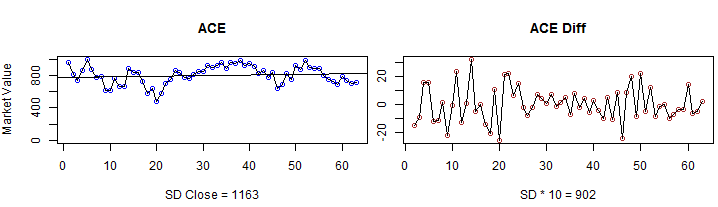
\includegraphics[width=1\textwidth]{images/chapter6/ACE_FRST.png}
        }\\
        \subfigure{
            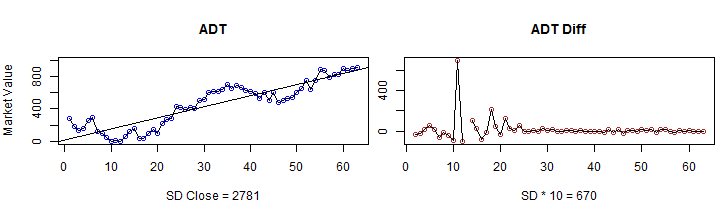
\includegraphics[width=1\textwidth]{images/chapter6/ADT_FRST.png}   
        }\\
        \subfigure{
            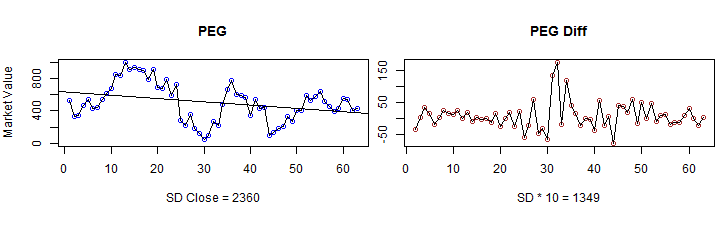
\includegraphics[width=1\textwidth]{images/chapter6/PEG_FRST.png}
        }\\
    \end{minipage}}
    \caption{Three samples of stocks's profiles of S\&P\,500 data set.}
    \label{fig:stockProfiles}
\end{figure}
    
    
    \subsubsection{Driving Classes from Stock's Profiles}
    \label{sec:Driving_Classes_from_Stock_Profiles}
To create classes for stocks, we used the visual profiles of the stocks to help experts to decide the final number of classes and the limits of each class. The very obvious classes are dividing the stocks into stable and unstable parts. However, after carefully examining classes, we can determine that the stable class can be further split into two classes: the very stable; and the rest. It is also true for the unstable class to be divided into two parts, the unstable and slightly stable classes. So, the final number of classes become four. They are:
    
\begin{itemize}
    \item \textbf{Very stable:} the price of this class of stocks experiences a relatively small change over time.
    
    \item \textbf{Smooth stable:} the price fluctuation of this class of stocks is larger than very stable class, with a small difference in price between two consecutive days on average.
    
    \item \textbf{Rough stable:} the price of this class of stocks is larger than that of the very stable class, with a large difference in price between two consecutive days on average.
    
    \item \textbf{Unstable:} the price of this class of stocks experiences relatively large changes over time.
\end{itemize}

While other class numbers might be possible, classifying stock market into four classes, however, gives it an advantage of becoming comparable with public goods games data set as it also has four classes.

The initial rules for classification were produced by human experts, with ranges in the forms of [min, max] values. Both aggregated attributes  generated in section \ref{sec:Approach_ch6} are used to express these rules. The rules are designed and prioritised so that the obvious stocks will be classified first (unstable and very stable), then rough stable stocks are labelled; finally, any remaining stock will be classified as smooth stable. The class rules with their priority order are shown in Table \ref{tab:InitialRulesStockMarket}. These rules will be optimised, and a single value will be chosen for each range. These are as described in the next subsection.

\begin{table}[!h]
    \ra{1.3}
    \small
    \centering
    \caption{Initial classification rules of stock market data set}
    \label{tab:InitialRulesStockMarket}
    \begin{tabular}{rl}
        \toprule
        \multicolumn{1}{c}{Class} & \multicolumn{1}{c}{\textbf{Rule}} \\ 
        
        \midrule
        
        \textbf{Very Stable} & stdevClose $ > $ [1100, 1300] \&\& stdevCloseDiff $ > $ [500, 750]   \\
        
        \textbf{Unstable}    & stdevClose $ < $ [1600, 2000] \&\& stdevCloseDiff $ < $ [650, 1000]   \\
        
        \textbf{Rouged Stable}                & stdevCloseDiff $ < $ [550, 800]        \\ 
        
        \textbf{Smooth Stable}                &  All remaining instance after the above filters (Others)                        \\
        \bottomrule 
    \end{tabular}
\end{table}

\subsection{Optimising Rules Using Heuristic}

Differential Evolution (DE) is a heuristic search algorithm introduced by Storn et al.  \cite{Storn1997}, who described it as simple and efficient. Differential Evolution is a type of evolutionary algorithm that uses crossover and mutation while producing the next generation. This happens according to the nature of DNA and derives natural evolution from creating solutions (species) that are optimised for the environment. This algorithm has proved to be successful, and it has been used in many different areas  \cite{Application2011}.  In this study, we used Differential Evolution to optimise provided rules by a human classifier. The optimisation focuses on minimising the distance between items within classes according to their temporal attributes. Please see chapter three for more details about DE.



\section{Testing With Public Goods Game Data Sets}
In this section, we will compare the results of classifying public goods games using brute force and differential evolution according to their speed and similarity. Then, we compare the proposed method with well-known classification methods such as ctree, SVM and c50. The comparison will be run on the 10 rounds of public goods games data set as it contains more players than the 27 rounds data set, as the number of items is more important for the training and testing of classifiers than longer time points. These two comparisons are necessary to demonstrate the ability of the proposed classification method to function in more of a general scope than only be restricted to the public goods games data sets with an acceptable efficiency of speed and accuracy.

\subsection{Comparing Brute Force and Heuristic Results}

The main advantage of using heuristic functions to solve the problem of optimisation is to reduce the required search time to find an optimum solution. However, it is important to check the heuristic function results to ensure that they are not radically different from the brute force results.

To accomplish the comparison, we use the differential evolution package \cite{Ardia2015} of R language. The maximum iteration is set on 200 iterations with 50 chromosomes in each generation. By default, the result of each iteration is real numbers. It can, however, be changed to produce only integer numbers. The speed and optimisation result of the algorithm is mainly dependent on the maximum-allowed number of iterations. For our tests, the average rounded speed of the results were 7 minutes compared to 48 for the brute force which makes it nearly seven times faster.

Table \ref{tab:bestPGG10DataSets_BF_DE} shows the optimum classification results of both brute force and differential evolution for different cost functions.  The four player classes are Free Rider FR, Weak Contributor WC, Normal Contributor NC and Strong Contributor SC. The optimum classification rules generated by the different methods are mostly similar with two exceptions:

\begin{itemize}
    \item The values for the rules of belief attribute for normal contributors are different for all cost functions.
    
    \item There are many differences between brute force generated rules and differential evolution ones for centroid distance cost function.
    
\end{itemize}

Despite these differences, Table \ref{tab:ClassMembership_BF_VS_DE} shows that there is no difference between classification results of both methods of optimisation except for the test where centroid distance is used as a cost function. From these two tables (Table \ref{tab:bestPGG10DataSets_BF_DE} and Table \ref{tab:ClassMembership_BF_VS_DE}) we can arrive at three conclusions:

\begin{landscape}
    \begin{table}[!h]
        
        \ra{1.3}
        \small
        \centering
        
        \caption{Comparing of brute force and differential evolution results for optimising attributes' values for the ranges of the initial classification rules of 10 rounds public goods games data set for different cost functions.}
        \label{tab:bestPGG10DataSets_BF_DE}
        \begin{tabular}{@{}crccccccccccccccccccccc@{}}
            \toprule
            
            & & \multicolumn{10}{c}{\textbf{Brute Force}}
            &  \phantom{abc} &
            \multicolumn{10}{c}{\textbf{Heuristics (DE)}}
            \\
            \cmidrule{3-12} \cmidrule{14-23}
            
            &    & \multicolumn{3}{c}{\textbf{$\overline{Contribution}$}} &  \phantom{a}& \multicolumn{3}{c}{\textbf{$\overline{Belief}$}} &  \phantom{a}& \multicolumn{2}{c}{\textbf{$\left |Zero\right |$}}
            
            &  \phantom{abc}&
            \multicolumn{3}{c}{\textbf{$\overline{Contribution}$}} &  \phantom{a}& \multicolumn{3}{c}{\textbf{$\overline{Belief}$}} &  \phantom{a}& \multicolumn{2}{c}{\textbf{$\left |Zero\right |$}} \\
            
            \cmidrule{3-5} \cmidrule{7-9} \cmidrule{11-12} \cmidrule{14-16} \cmidrule{18-20}  \cmidrule{22-23}
            
            &    & FR  & WC  & NC & \phantom{a} & FR & WC& NC & \phantom{a}& FR & WC  
            &  \phantom{abc}& 
            FR  & WC  & NC & \phantom{a} & FR & WC& NC & \phantom{a}& FR & WC
            \\ \midrule
            \multirow{2}{*}{\begin{turn}{90}{\scriptsize Statistics}\end{turn}}    
            & IQR & 
            1    & 3   & 5 & \phantom{a}           
            & 2  & 4   & 2 & \phantom{a}        
            & 6   & 5                         
            & \phantom{a} &
            1    & 3   & 5 & \phantom{a}           
            & 2  & 4   & \textcolor{red}{5} & \phantom{a}        
            & 6   & 5                         \\
            
            &Stdev & 
            1   & 1   & 6 & \phantom{a}           
            & 2  & 4  & 2  & \phantom{a}       
            & 9  & 6        
            & \phantom{a} &
            1    & 1   & 6 & \phantom{a}           
            & 2  & \textcolor{red}{9}   & \textcolor{red}{9} & \phantom{a}        
            & 9   & 6                         \\
            \midrule
            
            \multirow{2}{*}{\begin{turn}{90}{\scriptsize Euclidean}\end{turn}}
            &Complete & 
            1  & 3  & 6   & \phantom{a}           
            & 2  & 4  & 2   & \phantom{a}        
            & 7  & 5                         
            & \phantom{a} &
            1    & 3   & 6 & \phantom{a}           
            & 2  & 4   & \textcolor{red}{9} & \phantom{a}        
            & 7   & 5                         \\
            
            &Centroid & 
            1  & 2  & 2  & \phantom{a}           
            & 2  & 4  & 2       & \phantom{a}       
            & 6  & 5        
            & \phantom{a} &
            1    & \textcolor{red}{3}   & 2 & \phantom{a}           
            & \textcolor{red}{9}  & \textcolor{red}{6}   & \textcolor{red}{7} & \phantom{a}        
            & \textcolor{red}{8}   & 5                         \\
            
            \midrule
            
            \multirow{4}{*}{\begin{turn}{90}{\scriptsize ICVI }\end{turn}}
            & Dunn & 
            1  & 3  & 2 & \phantom{a}           
            & 7  & 7  & 2 & \phantom{a}        
            & 6  & 6            
            & \phantom{a} &
            1    & 3   & 2 & \phantom{a}           
            & \textcolor{red}{8}  & 7   & \textcolor{red}{6} & \phantom{a}        
            & 6   & 6                         \\
            
            &DB & 
            1  & 4  & 2 & \phantom{a}           
            & 2  & 5  & 2 & \phantom{a}        
            & 5  & 6        
            & \phantom{a} &
            1    & 4   & 2 & \phantom{a}           
            & 2  & 5   & \textcolor{red}{8} & \phantom{a}        
            & 5   & 6                         \\
            
            & SD & 
            1  & 4  & 6 & \phantom{a}           
            & 7  & 4  & 2 & \phantom{a}        
            & 9  & 6 
            & \phantom{a} &
            1    & 4   & 6 & \phantom{a}           
            & \textcolor{red}{8}  & 4   & \textcolor{red}{7} & \phantom{a}        
            & 9   & 6                         \\
            
            &S\_Dbw & 
            1  & 4  & 4 & \phantom{a}           
            & 2  & 4  & 2 & \phantom{a}        
            & 8  & 6        
            & \phantom{a} &
            1    & 4   & 4 & \phantom{a}           
            & 2  & 4   & \textcolor{red}{6} & \phantom{a}        
            & 8   & 6                         \\
            
            \bottomrule                        
        \end{tabular}
    \end{table}
\end{landscape}

\begin{itemize}
    
    \item The rule of the belief attribute for Normal Contributor class might be more flexible than accepting only one value, or it is irrelevant, and the rule can be further simplified.
    
    \item For the centroid-distance cost function, the heuristic failed to reach the most optimum value in 200 iterations as it did not generate the exact results as the brute force function. However, the result is not very far from the most optimum value as AUC measure of ROC analysis scored 0.94 which can be considered as an acceptable result.
    
    \item From the above, we can conclude that the differential evolution function can optimise the rules for the proposed classification at a faster rate with exact or acceptable results. Hence, we can use this heuristic method for future tests with larger data sets confident that it will produce an acceptable optimisation result.
    
\end{itemize}
\begin{table}[!h]
    \small
    \centering
    \caption{Comparing class membership results of the brute force and differential evolution in 10 rounds of public goods game data set using different cost functions.}
    \label{tab:ClassMembership_BF_VS_DE}
    \begin{tabular}{@{}crccccccccccccc@{}}
        \toprule
        &&& \multicolumn{4}{c}{Brute force} && \multicolumn{4}{c}{Heuristic (DE)}&&& \\
        &Cost Function &   & Fr  & Wc & Nc & Sc && Fr  & Wc & Nc & Sc && AUC & \\
        \midrule
        \multirow{2}{*}{\begin{turn}{90}{\scriptsize Statistics}\end{turn}}
        & IQR           && 46 & 22 & 22 & 50 && 46 & 22 & 22 & 50 && 1 & \\
        & Stdev         && 36 & 10 & 58 & 36 && 36 & 10 & 58 & 36 && 1 &  \\
        
        \midrule
        \multirow{2}{*}{\begin{turn}{90}{\scriptsize Euclidean}\end{turn}}
        & Complete      && 38  & 30 & 37 & 35 && 38  & 30 & 37 & 35 && 1 & \\
        & Centroid      && 46  & 10 & 0  & 84 && 30  & 25 & 6  & 79 && 0.94 & \\
        
        \midrule
        \multirow{4}{*}{\begin{turn}{90}{\scriptsize ICVI }\end{turn}}
        & Dunn          && 42 & 4  & 9  & 85 && 42 & 4  & 9  & 85 && 1 & \\
        & DB            && 37 & 34 & 2  & 67 && 37 & 34 & 2  & 67 && 1 & \\
        & SD            && 28 & 48 & 28 & 36 && 28 & 48 & 28 & 36 && 1 & \\
        & S\_Dbw        && 37 & 40 & 1  & 62 && 37 & 40 & 1  & 62 && 1 & \\
        \bottomrule
    \end{tabular}
\end{table}

\subsection{Comparing Results with Other Classification Methods}

In this section, we will test the proposed temporal classification method's ability to operate at a comparable efficiency (i.e. classifying items correctly) with general and popular classification algorithms. If we demonstrate the ability of the proposed classifier to classify items as effective as other classification algorithms, it might be an indication that the proposed algorithm can be used in more general areas rather than only be restricted to the public goods game data sets.

There are many classification methods which can operate on temporal data in various ways \cite{Amr2009}. However, we chose three classification methods to compare the proposed method with. The first classification method is Support Vector Machine \textbf{SVM}, which is one of the most successful classification algorithms  \cite{Bazi2006}. Besides its success, SVM is a partition based classification method which classifies items through creating hyperplanes between classes. This feature is similar to the initial rule construction of the proposed classification. The second classification method is C5.0 which is an extension of C4.5 which is, in turn, an extension of Iterative Dichotomiser 3 \textbf{ID3} \cite{Letham2010}. This algorithm was selected as the best algorithm for data mining and classification by \cite{Wu2008} for 2008 and ever since, its popularity and success have grown. This algorithm with all its variations is considered as a decision tree and rule-based classification method \cite{Giacometti2008} which makes it a perfect candidate for comparison with the proposed classification algorithm. The final classification algorithm is conditional inference trees \textbf{ctree} which is considered a statistical decision tree classifier. This algorithm uses tree-structured regression models to classify items in the data set \cite{Hothorn2006a}.

These classification methods were originally designed to work with none-temporal data sets. However, it is possible to use these classifiers with temporal data sets by preprocessing the temporal data before building the classification model \cite{Revesz2011}. There are multiple methods of extracting features from the temporal data in the preprocessing stage such as Singular Value Decomposition, Discrete Fourier Transform, Discrete Wavelet Transform and Piecewise Aggregate Approximation \cite{Zhao2014}. In this test, we will use Discrete Wavelet Transform which was introduced by Zhang et al. \cite{Zhang2004}, due to its popularity and acceptance in many areas which require temporal data mining \cite{Fu2011}. Moreover, it is also possible to use the plain temporal data of items directly for the tests by converting each time point into a separate feature (attribute) of the items. These attributes are created by transposing a single temporal attribute (i.e. contribution) which means for the 10 rounds data set 10 attributes are used, and 27 attributes are created for the 27 rounds of public goods game data set.

One of the advantages of the proposed classification method is its ability to classify items from optimised rules provided by a human expert. However, this might create a challenge when we want to assess it in comparison with other classification methods especially when these methods require pre-labelled data records to train their classifier model.

To be able to test the accuracy of these classification methods, we first use the existing labels which are provided by the economists. Although these labels are not based on the temporal data of the players, it might still offer a valuable insight into how well these labels are related to their temporal behaviour. The second types of labels are driven from the [min, max] attribute limits which are provided as initial rules by experts.  Instead of using optimisation for [min, max] pairs, we use the rounded average of each pair (i.e. the middle) as it might represent the best guess if the experts manually labelled the players. We use the average of the [min, max] spectrum because normal distribution is assumed for the players' contribution in the public goods games \cite{Itaya2010, Anderson1998}. Hence the natural dividing line between two classes might be in the middle of the spectrum.


\begin{table}[!h]
    \small
    \centering
    \centering
    \caption{AUC of ROC analysis for different classes and the proposed classification method of 10 rounds of public goods games.}
    \label{tab:ComparingClasses_10}
    \begin{tabular}{rcccccc}
        \toprule
        \multicolumn{1}{c}{\multirow{1}{*}{Classification}} &\phantom{a} 
        & \multicolumn{2}{c}{Labels}  &\phantom{abc} & \multicolumn{2}{c}{Classes} \\
        \cmidrule{3-4} \cmidrule{6-7}
        
        \multicolumn{1}{c}{\multirow{1}{*}{Method}} &\phantom{abc} 
        & \begin{tabular}{c} Temporal \\ attributes \end{tabular}
        & \begin{tabular}{c} DWT \\ attributes \end{tabular}  &\phantom{a} 
        & \begin{tabular}{c} Temporal \\ attributes \end{tabular} 
        & \begin{tabular}{c} DWT \\ attributes \end{tabular}        \\
        \midrule
        SVM     & \phantom{abc} & 0.602    & 0.504  &\phantom{a} & 0.877  & 0.797        \\
        Ctree   & \phantom{abc} & 0.704    & 0.583  &\phantom{a} & 0.841  & 0.848        \\
        C5.0    & \phantom{abc} & 0.735    & 0.654  &\phantom{a} & 0.858  & 0.892        \\
        
        \midrule
        Proposed &\phantom{abc}& IQR  & \multicolumn{2}{c}{Complet Dist}   & SD    &    \\
        &\phantom{abc} &0.959 & \multicolumn{2}{c}{0.965 }         & 0.972  &    \\
        \bottomrule
    \end{tabular}
\end{table}

We use 10 fold cross validation \cite{Kohavi1995a} to create 10 different classifier models for each classification algorithm by using 90\% of the players' data. Then we tested the models with the remaining 10\% of the data to detect the accuracy of the classifiers. These (90/10) portions of the players are randomly selected for each fold, and the 10\% of the test players are always different from one fold to another. We use this method as the number of players for both data sets are limited. In this way, we can repeat the test multiple times using the same data sets.

For the proposed classification method, we used the optimised rules which are generated by using all the data set without splitting them into training/test portions. These classes are used as the reference for comparing the accuracy of the classifiers, which are optimised by using only the training portion of the data, 90\% to classify the remaining 10\%. For these comparisons, we selected three cost functions: IQR, Complete Distance and SD.

\begin{table}[!h]
    \small
    \centering
    \centering
    \caption{AUC of ROC analysis for different classes and the proposed classification method of 27 rounds of public goods games.}
    \label{tab:ComparingClasses_27}
    \begin{tabular}{rcccccc}
        \toprule
        \multicolumn{1}{c}{\multirow{1}{*}{Classification}} &\phantom{a} 
        & \multicolumn{2}{c}{Labels}  &\phantom{abc} & \multicolumn{2}{c}{Classes} \\
        \cmidrule{3-4} \cmidrule{6-7}
        
        \multicolumn{1}{c}{\multirow{1}{*}{Method}} &\phantom{abc} 
        & \begin{tabular}{c} Temporal \\ attributes \end{tabular}
        & \begin{tabular}{c} DWT \\ attributes \end{tabular}  &\phantom{a} 
        & \begin{tabular}{c} Temporal \\ attributes \end{tabular} 
        & \begin{tabular}{c} DWT \\ attributes \end{tabular}        \\
        \midrule
        SVM     & \phantom{abc} & 0.658    & 0.495  &\phantom{a} & 0.819  & 0.725        \\
        Ctree   & \phantom{abc} & 0.665    & 0.5    &\phantom{a} & 0.781  & 0.864        \\
        C5.0    & \phantom{abc} & 0.597    & 0.671  &\phantom{a} & 0.852  & 0.818        \\
        
        \midrule
        Proposed &\phantom{abc}& IQR  & \multicolumn{2}{c}{Complet Dist}   & SD    &    \\
        &\phantom{abc}& 0.957 & \multicolumn{2}{c}{0.921 }         & 0.914  &    \\
        \bottomrule
    \end{tabular}
\end{table}

The AUC of the ROC analysis of all classification methods for both data sets are shown in Table \ref{tab:ComparingClasses_10} and Table \ref{tab:ComparingClasses_27}. The AUC results of classification models which are created based on the economists' labels score very low, especially with SVM and ctree. These results came as no surprise because the labels are not intended to represent the temporal behaviour of the players. The importance of these results is to present yet further evidence that the players change their strategy during the game and do not follow the static contribution table. This creates the need to classify players using their temporal contribution attributes directly.

We also used both data sets to create classifier models for the generated classes by using the experts' initial rules. It can be noticed that the average of AUC of the 10 fold cross-validation for each classification algorithm (SVM, ctree and C5.0) is less than (0.1). These results might be an indication that the different data sets (i.e. transposed and wavelet transformed for the temporal attribute) do not affect the accuracy of the classifier significantly for the public goods games data sets. 

The results from the proposed classification method using different cost functions produced a higher average of AUCs than the traditional classification methods. This result came as no surprise as these classification algorithms used classes which are produced by the average of the provided [min, max] while the proposed classification used the optimum value for each class limits. This means that the available classifiers are not necessarily performing worse than the proposed classification method. However, it might be an indication that optimising initial ranges for class rules provided by experts can perform better than when using crisp rules directly for classes. 

The results indicate that the proposed method can perform better than available common classification algorithms without sacrificing the understandability of the rules. As these algorithms might create complex models possibly incomprehensible for humans especially for temporal data sets, data transformation from time domain to frequency domain may be necessary. The clarity of the rules might lead to better understanding of the underlying data. This understanding might enable experts to provide even more accurate initial rules through multiple iterations of rule generation and optimisation as described in chapter five. On the other hand for complex data sets with the availability of well-established training data sets and accurate classes for the items (for example, classifying cancer cases using protein biomarkers  \cite{Liu2013}), it might be difficult for the experts to construct an efficient initial classifier by following the effects of hundreds of proteins.

\section{Testing Stock Market Stability}

To test the stability of the stock market and check the validity of Hypothesis  \ref{hypo:pridictabilityOfStocks}, we use the introduced data set in chapter three of Standard \& Poor's 500 (S\&P\,500) stock market. The whole data set contains stock records between 1-1-2015 to 1-7-2017. Two kinds of experiments are run on the data: In the first experiment, we measure stock changes over time for the first quarter using different references of behaviour to obtain an understanding of how stocks' stability changes over time. In the second experiment, we split the data into two parts; each part represents one quarter of the financial year. We used the first part to optimise a classifier based on the provided initial rules by the experts, and then we used this classifier to classify both quarters of the fiscal year to compare the class membership of each stock between these quarters and test the validity of Hypothesis  \ref{hypo:pridictabilityOfStocks}.

\subsection{Analysing Stocks' Behaviour}

To gain a better understanding of the presented stock market data set in chapter three and analyse the behaviour of the stocks between different time points, we measure changes over time for the entire stock market data using the proposed method in chapter three. Three different references of behaviour are used in the experiments: the first time point, the previous time point and the stocks' overall behaviour in the data set.


Each reference of behaviour can highlight different aspects of the stocks. By using the first time point as the reference of behaviour, we might be able to determine the level accuracy in predicting any future time point of the stock market by using the last available time point. Using the previous time point as the reference of behaviour, we can determine the stability of the stocks for the next day and hence, the ability to predict the stock market only for the next day. Using stocks' stability classes as the reference of behaviour, we can determine the overall stability of the stock market and its predictability in general.


Using the first and previous time points as references of behaviour are straight forward as these time points can be clustered alongside with other time points using one of the selected clustering algorithms (k--means, c--means, PAM and hierarchical). They can then be compared with other time points using external cluster validity indices as has been implemented in chapter four. However, to use the general behaviour of the stocks in the overall time points, they have to be classified according to their stability using their temporal attributes (closing price). To classify stocks in the data sets, we use the proposed rule-based temporal classification method. As explained beforehand, the proposed classification consists of two steps: initial rule generation and rule optimisation. We optimise the initial rules which are provided in section \ref{sec:Driving_Classes_from_Stock_Profiles}, Table \ref{tab:InitialRulesStockMarket}, by using Differential Evolution algorithm  to accelerate the process of rule optimisation. For this experiment, we used IQR as the cost function. The final rules are shown in Table \ref{tab:OptimisedRulesStockMarket} after optimisation.

\begin{table}[!h]
    \ra{1.3}
    \small
    \centering
    \caption{Optimised classification rules of stock market data set, using IQR as cost function for optimisation process.}
    \label{tab:OptimisedRulesStockMarket}
    \begin{tabular}{rl}
        \toprule
        \multicolumn{1}{c}{Class} & \multicolumn{1}{c}{\textbf{Rule}} \\ 
        
        \midrule
        
        \textbf{Very Stable} & stdevClose $ > $ 1246 \&\& stdevCloseDiff $ > $ 584   \\
        
        \textbf{Unstable}    & stdevClose $ < $ 1996 \&\& stdevCloseDiff $ < $ 797   \\
        
        \textbf{Rouged Stable}                & stdevCloseDiff $ < $ 759        \\ 
        
        \textbf{Smooth Stable}                &  All remains                        \\
        \bottomrule 
    \end{tabular}
\end{table}

Figure \ref{fig:ChangeMeasuers_First_Stock} shows the results of the change in the stocks over time compared with the first time point. The stocks are clustered in each time point using different clustering algorithms (k--means, c--means, PAM, hierarchical) and then compared with the first time point by various external cluster validity criteria (Rand, Jaccard, FM, VI and AUC). It can be noticed that the results for all clustering algorithms show a rapid change of stocks' clusters between the first time point and other consecutive time points until it nearly reaches the 20th time point. It then starts to straighten with some minor changes. This is an indication that further the distance from the current time point will produce less accurate predictions as the changes over time become more significant until the saturation point is reached near the 20th time point. At that point (20th), changes in the stock market cancel each other out. We can, therefore, see this stability in much lower rates of similarity.

\begin{figure}[!h]
\hfill{\begin{minipage}{\dimexpr \textwidth-2\fboxsep-2\fboxrule}% maximum allowed
        \centering
        \subfigure[K--means Clustering]{
            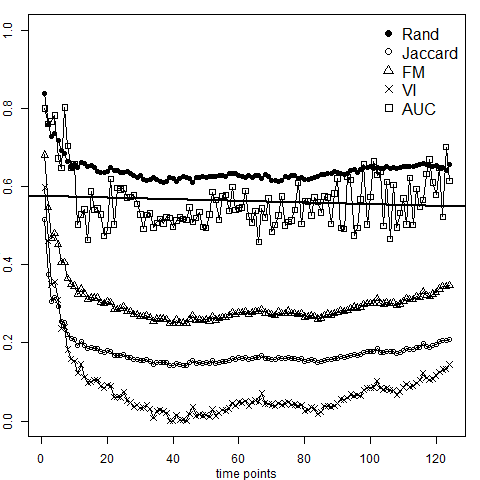
\includegraphics[width=0.45\textwidth]{images/chapter6/stock_kmeansClusters_Firs.png}
        }
        \subfigure[PAM Clustering]{
            \includegraphics[width=0.45\textwidth]{images/chapter6/stock_PAMClusters_Firs.png}
        }\\
        
        \centering
        \subfigure[C--means Clustering]{
            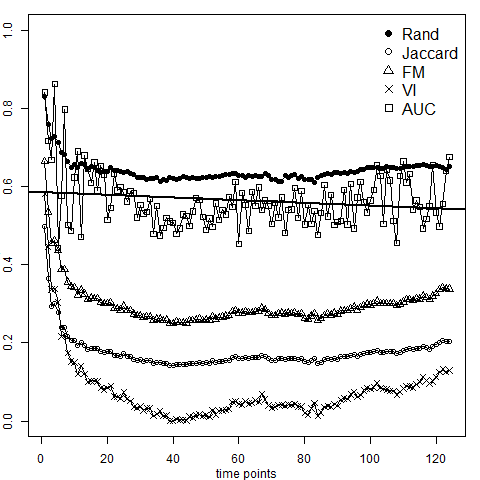
\includegraphics[width=0.45\textwidth]{images/chapter6/stock_cmeansClusters_Firs.png}
        }
        \subfigure[Hierarchical Clustering]{
            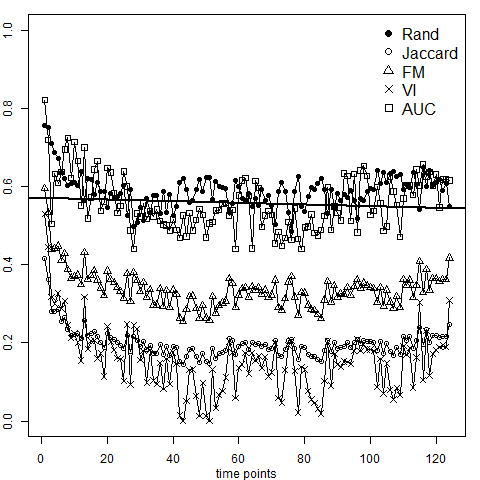
\includegraphics[width=0.45\textwidth]{images/chapter6/stock_hierClusters_Firs.png}
        }\\
        
    \end{minipage}}
    \caption{Using the first time point as reference of behaviour.}
    \label{fig:ChangeMeasuers_First_Stock}
\end{figure}

Figure \ref{fig:ChangeMeasuers_Cons_Stock} shows the results of the change between in stocks every current and next time points. The similarity between every consequent time point is high as indicated by the high regression line for the AUC measure. It can be noticed that, despite the high regression line, there is a sharp transition between any time point. This might be an indication that the overall stability classes do not change significantly between any two time points. However, individual stocks might change their classes more rapidly. This means that the overall status of the stock market can be predictable for the next day. However, individual stocks might not follow the trend of their class.

\begin{figure}[!h]
\hfill{\begin{minipage}{\dimexpr \textwidth-2\fboxsep-2\fboxrule}% maximum allowed
        \centering
        \subfigure[K--means Clustering]{
            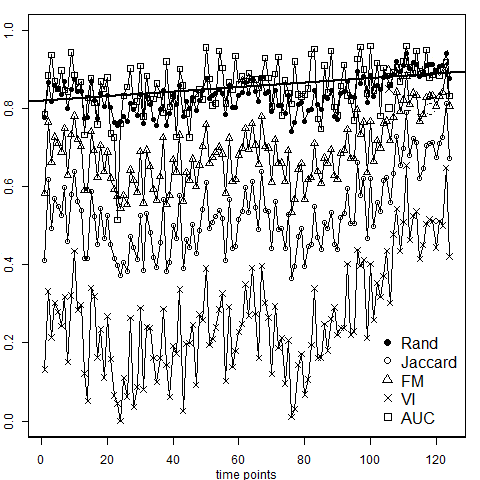
\includegraphics[width=0.45\textwidth]{images/chapter6/stock_kmeansClusters_Cons.png}
        }
        \subfigure[PAM Clustering]{
            \includegraphics[width=0.45\textwidth]{images/chapter6/stock_PAMClusters_Cons.png}
        }\\
        
        \centering
        \subfigure[C--means Clustering]{
            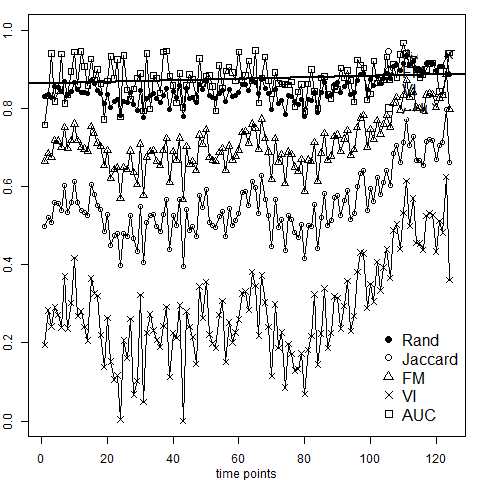
\includegraphics[width=0.45\textwidth]{images/chapter6/stock_cmeansClusters_Cons.png}
        }
        \subfigure[Hierarchical Clustering]{
            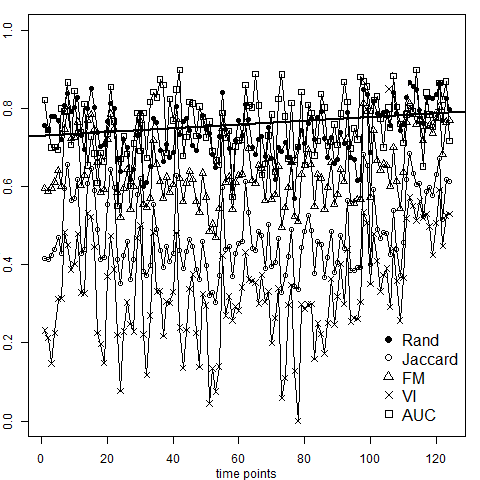
\includegraphics[width=0.45\textwidth]{images/chapter6/stock_hierClusters_Cons.png}
        }\\
        
    \end{minipage}}
    \caption{Using the previous time point as the reference of behaviour.}
    \label{fig:ChangeMeasuers_Cons_Stock}
\end{figure}

Figure \ref{fig:ChangeMeasuers_Cons_Stock} shows the results of the change in stocks over time compared with their overall stability classes. From the results, we can determine that there is a consistent difference between stocks' classes and their temporal behaviour. However, the difference is rather large. For example, the regression line for AUC is near 0.5 for all clustering methods, although it is flat. That is, its slope is close to zero.  This might be an indication that it is difficult to predict stocks by only using their overall past behaviour.


\begin{figure}[!h]
\hfill{\begin{minipage}{\dimexpr \textwidth-2\fboxsep-2\fboxrule}% maximum allowed
        \centering
        \subfigure[K--means Clustering]{
            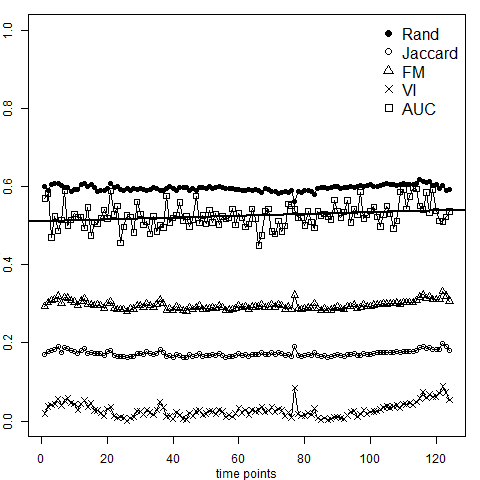
\includegraphics[width=0.45\textwidth]{images/chapter6/stock_kmeansClusters_Class.png}
        }
        \subfigure[PAM Clustering]{
            \includegraphics[width=0.45\textwidth]{images/chapter6/stock_PAMClusters_Class.png}
        }\\
        
        \centering
        \subfigure[C--means Clustering]{
            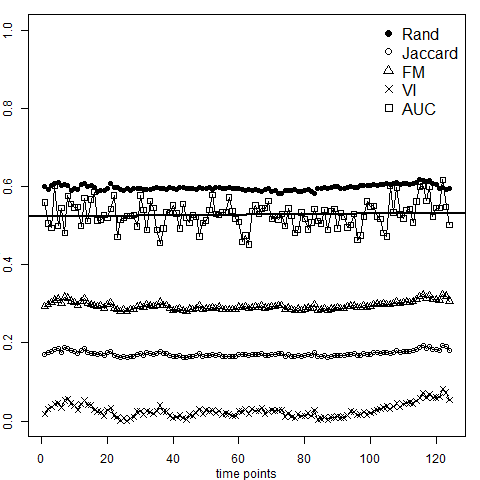
\includegraphics[width=0.45\textwidth]{images/chapter6/stock_cmeansClusters_Class.png}
        }
        \subfigure[Hierarchical Clustering]{
            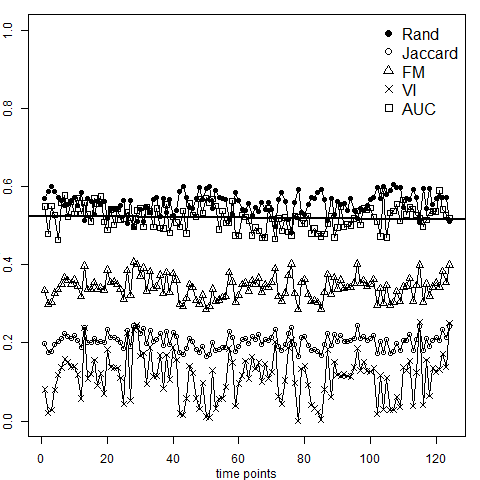
\includegraphics[width=0.45\textwidth]{images/chapter6/stock_hierClusters_Class.png}
        }\\
        
    \end{minipage}}
    \caption{Using the proposed classes as reference of behaviour.}
    \label{fig:ChangeMeasuers_Class_Stock}
\end{figure}

The three results achieved by comparing stock market behaviour by using different reference of behaviours lead us to conclude that it might be possible to predict stock market prices for the next day reasonably accurately. However, the accuracy of the prediction rapidly becomes lower for each other next day until it gets to a point where it might be equivalent to a random guess. This finding is aligned with the random walk hypothesis in stock market predictability which is supported by a group of economists  \cite{Fama1965}. This hypothesis states that the further walking away from a known stock price there is, the more inaccurate the prediction will become.


\subsection{Comparing Stocks' Class Memberships}

To verify Hypothesis \ref{hypo:pridictabilityOfStocks} and further check the ability to predict stock price by solely using historical prices of the stocks. We conduct an experiment to compare stocks' membership to one of the proposed stability classes (very-stable VS, smooth-stable SS, rough-stable RS, and the unstable US) in two consequent quarters of the fiscal year. If the majority of the stocks are classified as the same class for both quarters, Hypothesis ref{hypo:pridictabilityOfStocks} is valid. This then might be an indication that the first quarter's price can be used to predict the second quarter. In this experiment, we only test the ability of any prediction system to predict the market price for the next quarter, and not for the price the next day. Moreover, the test is solely concerned about predictors which use previous price data for their predictions, and not any other factors \cite{Agrawal2013}.

The first quarter's closing price of stocks is used to optimise the initial rules which are derived from profiles of stocks in section \ref{sec:Driving_Classes_from_Stock_Profiles}. Different cost functions are used in the optimisation process (Stdev, IQR, and Complete Distance) so that various classifiers are produced. The optimised classifiers are used to classify both quarters separately. Then the class membership of stocks in both quarters is compared to calculate the percentage of the stocks with identical classes in both quarters. Table \ref{tab:TemporalClassificationResult} shows the percentage and the number of stocks in each class in both quarters. The three results indicate that the majority of the stocks do not necessarily follow the same stability class in both quarters. 

\begin{table}[!h]
    \centering
    \caption{Number of stocks in each class and percentage of compatible results between two quarters of the fiscal year using different cost functions}
    \label{tab:TemporalClassificationResult}
    \begin{tabular}{rcccccc}
        \hline
        \multirow{2}{*}{\begin{tabular}[c]{@{}c@{}}Compactness\\ Measures\end{tabular}} & \multirow{2}{*}{Quarters} & \multicolumn{4}{c}{Items in Classes/Clusters} & 
        \multirow{2}{*}{\begin{tabular}[c]{@{}c@{}}Quarters\\ Agreement \end{tabular}} \\ \cline{3-6}
        &        & VS         & US         & RS        & SS        &  \\ \hline
        
        \multirow{2}{*}{Stdev} 
        &  Qt1 & 42   & 172  & 99  & 184  & \multirow{2}{*}{34\%}   \\ 
        &  Qt2 & 112  & 59   & 79  & 247  &  \\ \hline
        
        \multirow{2}{*}{IQR}
        & Qt1  & 87  & 245  & 30   & 135  & \multirow{2}{*}{37\%} \\ 
        & Qt2  & 197 & 119  & 19   & 162  &  \\ \hline
        
        \multirow{2}{*}{Complete Dist} 
        & Qt1  & 120  & 123  & 128 & 126  & \multirow{2}{*}{34\%}  \\ 
        & Qt2  & 242  & 43   & 83  & 129  & \\ \hline
    \end{tabular}
\end{table}

To compare the results of the stock classification in both quarters and confirm the results, we used various clustering algorithms to cluster each quarter separately. We then calculated the percentage of the stocks in the same cluster in both fiscal years' quarters. However, the percentage of agreement between clusters might not be sufficient for clustering methods due to the risk of instability of cluster labels. So, two external cluster validity indices (Jaccard index and Folkes-Mallows FM-index) are also used to measure the similarities between clusterings of the two quarters of the fiscal year. Three methods of clustering are used for this experiment, and they are:
\begin{itemize}
    
    \item K--means for aggregated attributes: In this method, we used k--means with two aggregated attributes which are derived from 'close' attribute. The attributes are 'StdevClose' which is the standard deviation of the close attribute for each item and StdevCloseDiff which is the standard deviation of closing price differences every two days. Please refer to section \ref{sec:Approach_ch6}for more information.
    
    \item K--means for temporal attributes: In this method, we used the transposed close attribute with k--means clustering. By transposing the close attribute, each time point of the temporal data become a separate attribute and contributes in the computation of choosing the optimum cluster for the stocks.
    
    \item Hierarchical for temporal attributes: In this method, we use hierarchical clustering with the 'close' temporal attribute directly by using Dynamic Time Wrapping DTW \cite{Berndt1994} distance. This method is more advantageous then Euclidean distance, and for time series data sets, it is less subject to time distortion.
    
\end{itemize}

The results in Table \ref{tab:TemporalClusteringResult} shows that the stocks in similar clusters for both quarters of the financial year are less than 50\%. This can also be seen in the results of the Jaccard and FM indices. It can be noticed that the hierarchical clustering using dynamic time wrapping is noticeably high (47\%). This may be the effect of the DTW. However, this high percentage of similarity result between two clusters might not be a representative figure as the dynamic time wrapping method shifts the time of items to find the smallest possible distance between two stocks' prices. However, this shift distorts the actual time of price change, which is crucial in the stock market data set.

\begin{table}[!h]
    \centering
    \caption{Number of stocks in each cluster and the percentage of compatible results between two quarters using different clustering methods.}
    \label{tab:TemporalClusteringResult}
    \begin{tabular}{rcccccccc}
        \hline
        
        Clustering Methods &   & Cl1   & Cl2 & Cl3  & Cl4   & Jaccard  & FM & \% \\ \hline
        
        \multirow{2}{*}{\begin{tabular}[r]{@{}r@{}}k--means\\ Aggregated\end{tabular}}
        & Qt1 & 89   & 81  & 176 & 151  
        & \multirow{2}{*}{0.17} & \multirow{2}{*}{0.30} & \multirow{2}{*}{27}  \\ 
        & Qt2 & 175  & 34  & 182 & 106  & &&  \\ \hline
        
        \multirow{2}{*}{\begin{tabular}[r]{@{}r@{}}k--means\\ Temporal\end{tabular}} 
        & Qt1  & 141   & 155  & 83  & 118 
        & \multirow{2}{*}{0.28} & \multirow{2}{*}{0.43} & \multirow{2}{*}{16}          \\ 
        & Qt2  & 53    & 138  & 164 & 142 & & & \\ \hline
        
        
        \multirow{2}{*}{\begin{tabular}[r]{@{}r@{}} Hierarchical\\ Temporal(DTW) \end{tabular}}   
        & Qt1  & 103   & 134   & 191  & 69  
        & \multirow{2}{*}{0.31}& \multirow{2}{*}{0.48}& \multirow{2}{*}{47}  \\ 
        & Qt2  & 102   & 251   & 113  & 31  & & & \\ \hline
    \end{tabular}
\end{table}


The results of both classification and clustering methods show the stability of stock price between the first and second quarters of the fiscal year are less than 50\%. This might suggest different stability behaviour for each stock price. This is an indication that Hypothesis \ref{hypo:pridictabilityOfStocks} has not been proven, which means it might not be possible to use one quarter's stock prices to predict the next quarter's prices. This conclusion does not include predicting the next day prices either using other factors to enhance the accuracy of the prediction.

\section{Summary}

In this chapter, we answered the question of stock market predictability only using prices of stocks by verifying the validity of Hypothesis 6. According to this hypothesis, 50\% of stock market prices do follow the same classification of their stability. To validate this hypothesis, we had to classify stocks according to their stability. However, the harvested data for this purpose have no pre-classified labels according to their stability.

To classify the stock market data set, we used the proposed rule-based temporal classification. However, this method had only been used to classify public goods games data set beforehand. To be able to use this classification method, we had to adjust its speed so that it can classify larger data sets, that is,  more items in the data set and longer time points. We replaced the brute force optimisation with differential evolution, which might shorten the required time for the optimisation process. Moreover, to be able to use the proposed method in more general areas than solely public goods games, we had to demonstrate that the produced classifier after the optimisation process is comparable to the brute force method and with other more general classification methods such as SVM, ctree, and C5.0.

We used the 10-round public goods games data set to compare results of both the brute force and differential evolution algorithm. The optimised classifiers had limited differences which ultimately did not affect the final result of classifying players, except slightly in the case of using the Euclidean distance of items from classes centroid as a cost function.

We then used both data sets of public goods games to compare results between three popular classifiers and the proposed method. We used two different sets of data attributes: 1none-temporal, contribution table attributes and 2temporal contribution and belief attributes. Furthermore, we used different labels to train the classifier models for each set of attributes as we used the economist's labels with non-temporal attributes and the midpoint between every [min, max] rule of the initial rules presented by the experts using player profiles. In all cases, the proposed classification method performed better than other classifiers; this might be mainly due to the advantage of optimising the rules which are presented by the experts instead of directly using labels to train classifiers. However, as we have argued before, for a data set with complex attributes and a sufficient training data set, the proposed classification method might not be so advantageous when used.

By using profiles of the stocks for their price behaviour, four classes are created: 1) stable, 2) smooth stable, 3) rough stable and 4) unstable. Initial rules for each class are created using aggregated attributes derived from the close price of the stocks. These rules contained a range of [min, max] values which had to be later optimised by using differential evolution to find the best classifier according to one of the available cost functions.

Before validating Hypothesis \ref{hypo:pridictabilityOfStocks}, we studied stock market behaviour in the data set using the proposed method for measuring changes over time in temporal data sets. Three different references of behaviour were used for this purpose: 1first time point, 2previous time point, and 3temporal class of the stocks. The first two references of behaviours were clustered alongside other time points for the comparison, while for the last one the proposed classification method is used to classify the stocks according to their price.

Different clustering methods were used to cluster stocks in each time point. Moreover, external cluster validity indices were used to measure the differences between each time point and its reference of behaviour.   It might be concluded from the results that the stock price similarity drops from each next day until it gets to a point before then starting to level out.

To validate Hypothesis \ref{hypo:pridictabilityOfStocks}, three different cost functions were used the first part of the data set, which represents one quarter, to optimise initial classification rules. Then, we classified both quarters with the optimised classifiers to produce class labels for each stock according to their stability in each quarter separately. After that, we computed the percentage of stocks with the identical classes in both quarters. The results suggested that under 50\% of the stocks have similar classes in both quarters.  This might be an indication that Hypothesis \ref{hypo:pridictabilityOfStocks} has not been proven and it is not possible to predict stocks behaviour in one quarter based on the previous quarter's price. This result was confirmed by using different clustering methods to cluster stocks in both quarters of the fiscal year as the results also suggested that most of the stocks not follow the same group in both cases.


